\section{SCARS Documentation}\label{sec:documentation}
    \dots\textit{implementation}\dots
    


    \subsection{Folder Structure}
        \dots\textit{work in progress}\dots
    


    \subsection{MATLAB Scripts}
        Along with Simulink models, SCARS is shipped with few MATLAB scripts. Their aim is to automate menial tasks that have to be performed by the user. Since the scripts guide the user with interactive prompts, there is no need for detailed documentation, just explanation of their purpose, presented in the list below:
        \begin{itemize}
            \item \verb|scarsSetup| - 
            \item \verb|getSunPosition| - 
            \item \verb|createSTKFiles| - 
            \item \verb|getSISOSystem| - 
        \end{itemize}
        
        \dots\textit{work in progress}\dots



    \subsection{Simulink Models Masks}
        Each model included in \ac{scars} Parts Library is masked with Simulink mask\cite{masks}. This allows the user to open custom interface for selected SCARS block, with editable fields for each parameter used in the setup process of that part. Most importantly, masks contain the description of the block. In case of SCARS, if the block represents a piece of hardware, the description contains short explanation of principle of operation of said part, its purpose within AOCS subsystem, notes about parameters, and description of block's inputs and outputs. In this way, majority of SCARS documentation is attached to the model itself, where it is easily accessible. An example of SCARS block mask can be found in figure \autoref{fig:model_mask}.
        
        \begin{figure}[H]
            \centering
            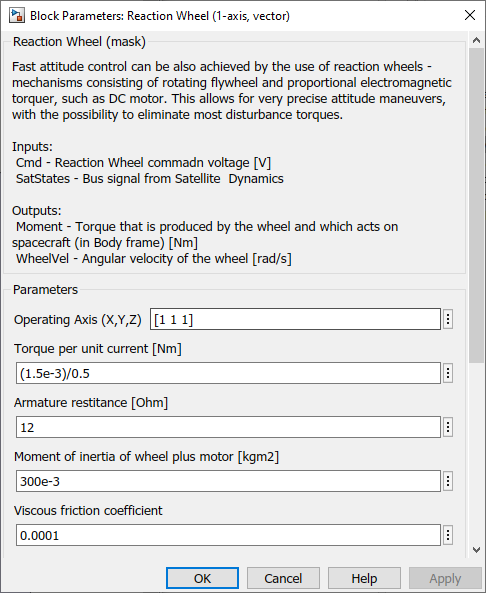
\includegraphics[width=1\textwidth]{3-documentation/rw_mask.png}
            \caption{SCARS Reaction Wheel mode; mssk}
            \label{fig:model_mask}
        \end{figure}
        
        Also, Simulink masks contain pieces of MATLAB code, which is executed after adding or changing the block. This code allows further customization of the initialization process. For example, \textbf{Reaction Wheel (1 axis, vector)} model transforms the vector given as axis of operation into its norm, "sanitating" user's input\cite{input_sanitization}. 
        % \dots\textit{description}\dots
